\documentclass[aspectratio=169,10pt]{beamer}
\usepackage{amsmath,amssymb}
\usepackage{graphicx}
\usepackage{booktabs}

\usetheme{default}
\setbeamertemplate{navigation symbols}{}
\setbeamertemplate{footline}[frame number]
\setbeamerfont{frametitle}{size=\large,series=\bfseries}
\setbeamertemplate{itemize items}[circle]
\setlength{\leftmargini}{1.2em}

% figures and numbers are written by the pipeline to outputs/
\graphicspath{{../outputs/}{outputs/}}
\newcommand{\resultsinput}[1]{%
  \IfFileExists{../outputs/tables/#1}{\input{../outputs/tables/#1}}{\input{outputs/tables/#1}}}
\newcommand{\given}{\,|\,}

\begin{document}
\resultsinput{bvd_numbers.tex}

% ---------------------------------------------------------------------------
\begin{frame}{Bundibugyo virus disease, 2026: how many cases are there really?}
\begin{columns}[T]
\begin{column}{0.47\textwidth}
\textbf{Data.} 44 situation reports, 12 July to 1 October. Each gives
confirmed cases by date of symptom onset: $C(t\given t')$, cases with onset
on day $t$ as shown in the report of day $t'$.

\medskip
\textbf{The difficulty.}
\begin{itemize}
\item Cases are reported with a delay, so recent counts are incomplete and the
epidemic curve always appears to be falling.
\item Counts are revised, occasionally downwards.
\item Reports are uneven: more on some days of the week.
\end{itemize}

\medskip
\textbf{Aim.} The true cases $I(t)$ and the reproduction number $R_t$, with
honest uncertainty, from the reports available on a given day.

\medskip
\textbf{Approach.} A joint model of transmission and of reporting, with the
$I(t)$ as unknowns. It extends Bajaj, Thompson \& Lambert (2025).
\end{column}
\begin{column}{0.53\textwidth}
\centering
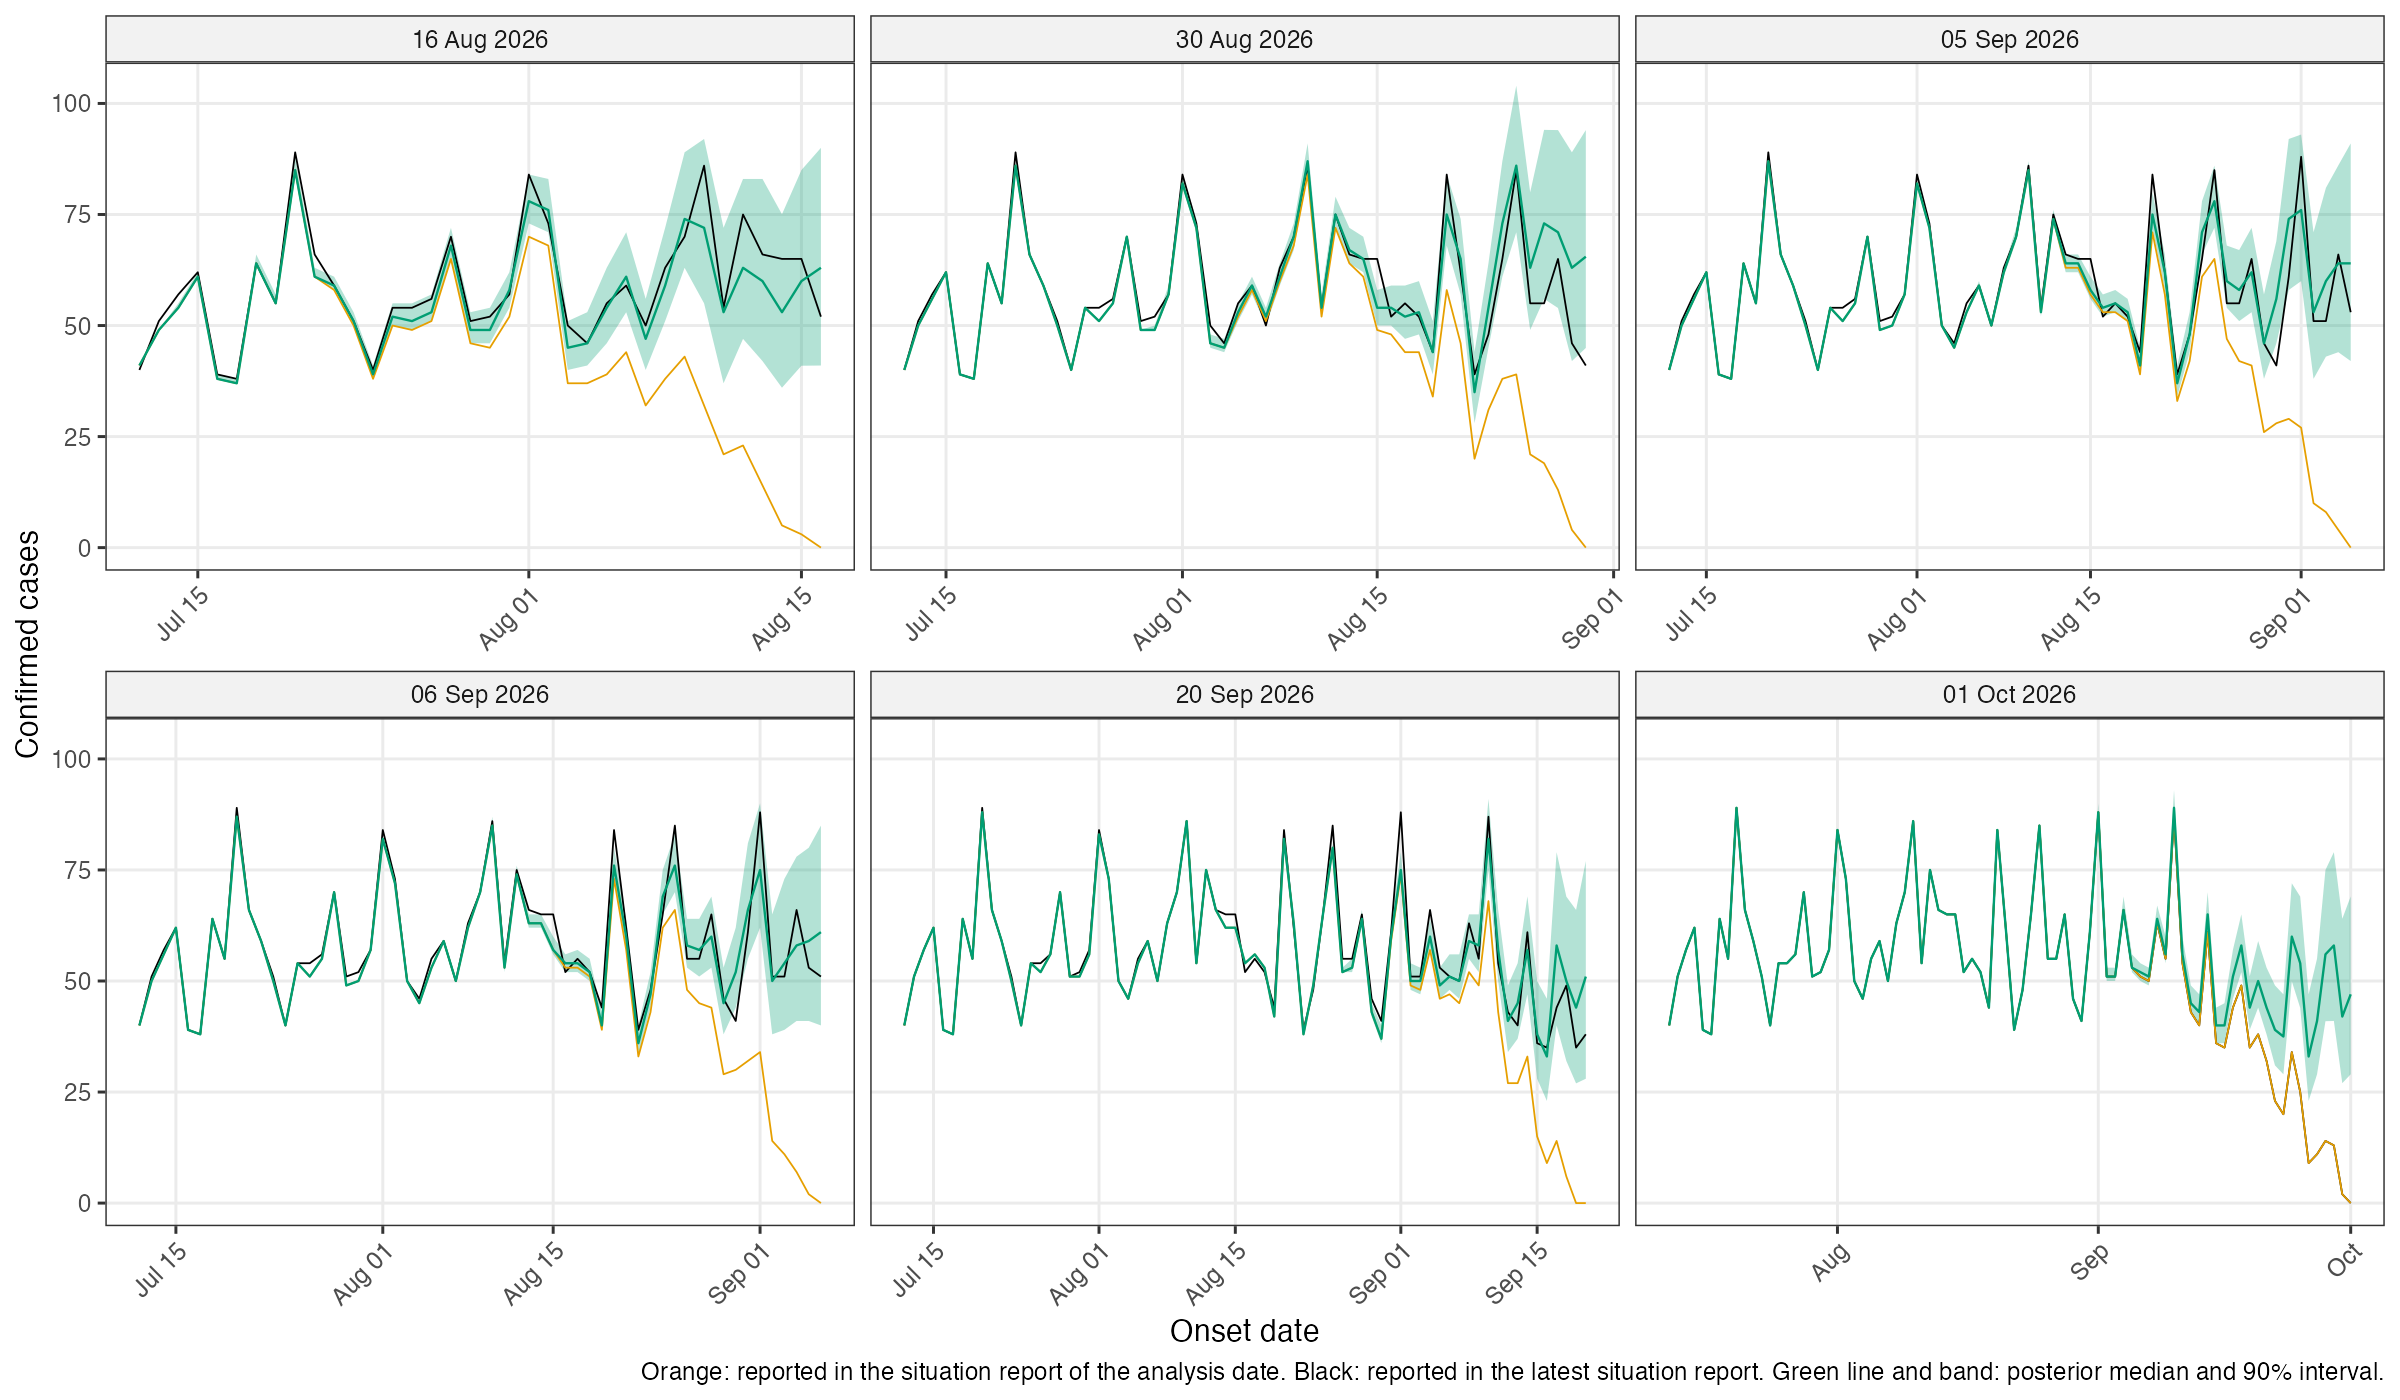
\includegraphics[width=\textwidth]{bvd_changepoint_cases.png}

{\footnotesize Orange: reported on the analysis date. Black: reported on 1
October. Green: estimated then.}
\end{column}
\end{columns}
\end{frame}

% ---------------------------------------------------------------------------
\begin{frame}{Model of transmission: a renewal process with changes at unknown times}
\begin{columns}[T]
\begin{column}{0.5\textwidth}
\textbf{Renewal equation}, overdispersed:
\[
I(t)\sim\operatorname{NB}\bigl(R_t\Lambda_t,\ \kappa\bigr),\qquad
\Lambda_t=\sum_{s=1}^{40}\omega_s\,I(t-s)
\]
\begin{itemize}
\item $\omega_s$: discretised gamma serial interval (mean 15.3, sd 9.3 days,
from Zaire ebolavirus).
\item Cases before the first report enter $\Lambda_t$ as known.
\end{itemize}

\medskip
\textbf{$R_t$ is piecewise constant}, with the number and positions of the
changes unknown. Segment values $R_j\sim\operatorname{gamma}(1,1)$.
\end{column}
\begin{column}{0.5\textwidth}
\textbf{Prior on the partition} (a product partition model; Barry \& Hartigan
1992): each day starts a new segment with probability $p$,
\[
p(\tau_1,\dots,\tau_K\given p)\propto p^{K}(1-p)^{T-1-K},\quad
p\sim\operatorname{beta}(1,T)
\]
with every segment at least 7 days.

\medskip
Integrating out $p$, a partition with $K$ changes has weight
$B(1+K,\,2T-1-K)$. Counting partitions:

\smallskip
\centering
{\small
\begin{tabular}{lcccc}
\toprule
Changes & 0 & 1 & 2 & $\ge 3$ \\
\midrule
Prior probability & 0.61 & 0.26 & 0.09 & 0.04 \\
\bottomrule
\end{tabular}}

\raggedright
\smallskip
The prior favours no change, and the penalty for a further change adapts to
the data through $p$.
\end{column}
\end{columns}
\end{frame}

% ---------------------------------------------------------------------------
\begin{frame}{Model of reporting: delays, days of the week and corrections}
\begin{columns}[T]
\begin{column}{0.5\textwidth}
\textbf{Delay.} Onset to report is gamma$(\mu,\sigma)$, with survival function
$S_\theta$. The delay parameters are also piecewise constant in onset day,
with the same prior on changes (segments of at least 14 days) and
\[
\log\mu_j\sim N(\log\mu_0,s^2),\quad \log\sigma_j\sim N(\log\sigma_0,s^2).
\]

\textbf{Day of the week.} The daily hazard of reporting is multiplied by
$\psi_w$, $w$ being the weekday of the report in which the case would first
appear:
\[
S^{*}_\theta(t\given t')=S_\theta(t\given t)
\exp\Bigl\{-\textstyle\sum_{k=t+1}^{t'}m_k\,h_\theta(t,k)\Bigr\}.
\]
\end{column}
\begin{column}{0.5\textwidth}
\textbf{Reported counts.} Between consecutive reports $t_{j-1}<t_j$, for
onset day $t$:
\begin{align*}
\text{genuine, first reported:}\quad & d_j\sim\operatorname{binomial}\bigl(I(t)-D_{j-1},\,p_j\bigr)\\
\text{records added in error:}\quad & n_j\sim\operatorname{Poisson}\bigl(\eta\,I(t)\,\Delta S^{*}_j\bigr)\\
\text{errors removed:}\quad & e_j\sim\operatorname{binomial}\bigl(E_{j-1},\,1-(1-\rho)^{\Delta t_j}\bigr)
\end{align*}
\[
C(t\given t_j)-C(t\given t_{j-1})=d_j+n_j-e_j
\]
with $p_j=1-S^{*}_\theta(t\given t_j)/S^{*}_\theta(t\given t_{j-1})$.

\medskip
$D$ (genuine cases reported) and $E$ (errors currently in the count) are
latent; $E$ is small and is summed out by a forward recursion.

\medskip
With $\eta=0$, $\psi_w=1$ and no changes, this is the original model, in which
counts can only rise.
\end{column}
\end{columns}
\end{frame}

% ---------------------------------------------------------------------------
\begin{frame}{Inference and checking}
\begin{columns}[T]
\begin{column}{0.5\textwidth}
\textbf{Sampler} (Metropolis within Gibbs; \bvdChains{} chains of
\bvdIterations{}):
\begin{itemize}
\item $I(t)$: each drawn from its discrete full conditional.
\item $R_t$ segments: with $R_j$ integrated out, the partition is drawn
\emph{exactly} by a forward recursion over segment starts, then the $R_j$.
No reversible-jump proposals.
\item Delay segments: split, merge and shift moves.
\item $\kappa,\psi_w,\eta,\rho$: random-walk Metropolis.
\end{itemize}

\medskip
\textbf{Convergence.} Largest split-$\widehat R$ across six analysis dates:
\bvdRhatCoreMax{} for cases and $R_t$; \bvdRhatDelayMeanMax{} for the delay;
\bvdRhatWeekdayMax{} for $\psi_w$.

\medskip
\textbf{Cross-check.} A continuous relaxation in Stan (NUTS), with the
change days summed out as a left-to-right hidden Markov model, gives the same
$R_t$ and the same probability of no change.
\end{column}
\begin{column}{0.5\textwidth}
\textbf{Posterior predictive checks} (replicated reports given each draw):

\smallskip
{\small
\begin{tabular}{lc}
\toprule
Statistic & $p$ \\
\midrule
Reported within 3 days of onset & \bvdPthree \\
Reported within 7 days & \bvdPseven \\
Reported within 14 days & \bvdPfourteen \\
Variation between reports in cases added & \bvdPvariation \\
Dispersion of cases about renewal mean & \bvdPdispersion \\
Variation by weekday of onset & \bvdPweekdayOnset \\
\bottomrule
\end{tabular}}

\medskip
\begin{itemize}
\item Transmission is described adequately.
\item Reporting: a small misfit in the gamma shape.
\item Estimates made on five earlier dates: 90\% intervals covered
\bvdCoverageMin{} to \bvdCoverageMax{} of the counts reported later; bias at
most \bvdBiasMax.
\end{itemize}

\medskip
{\footnotesize Leaving out cases before the first report made the dispersion
check fail badly: the misfit was absorbed as overdispersion.}
\end{column}
\end{columns}
\end{frame}

% ---------------------------------------------------------------------------
\begin{frame}{Results as of 1 October 2026}
\begin{columns}[T]
\begin{column}{0.66\textwidth}
\centering
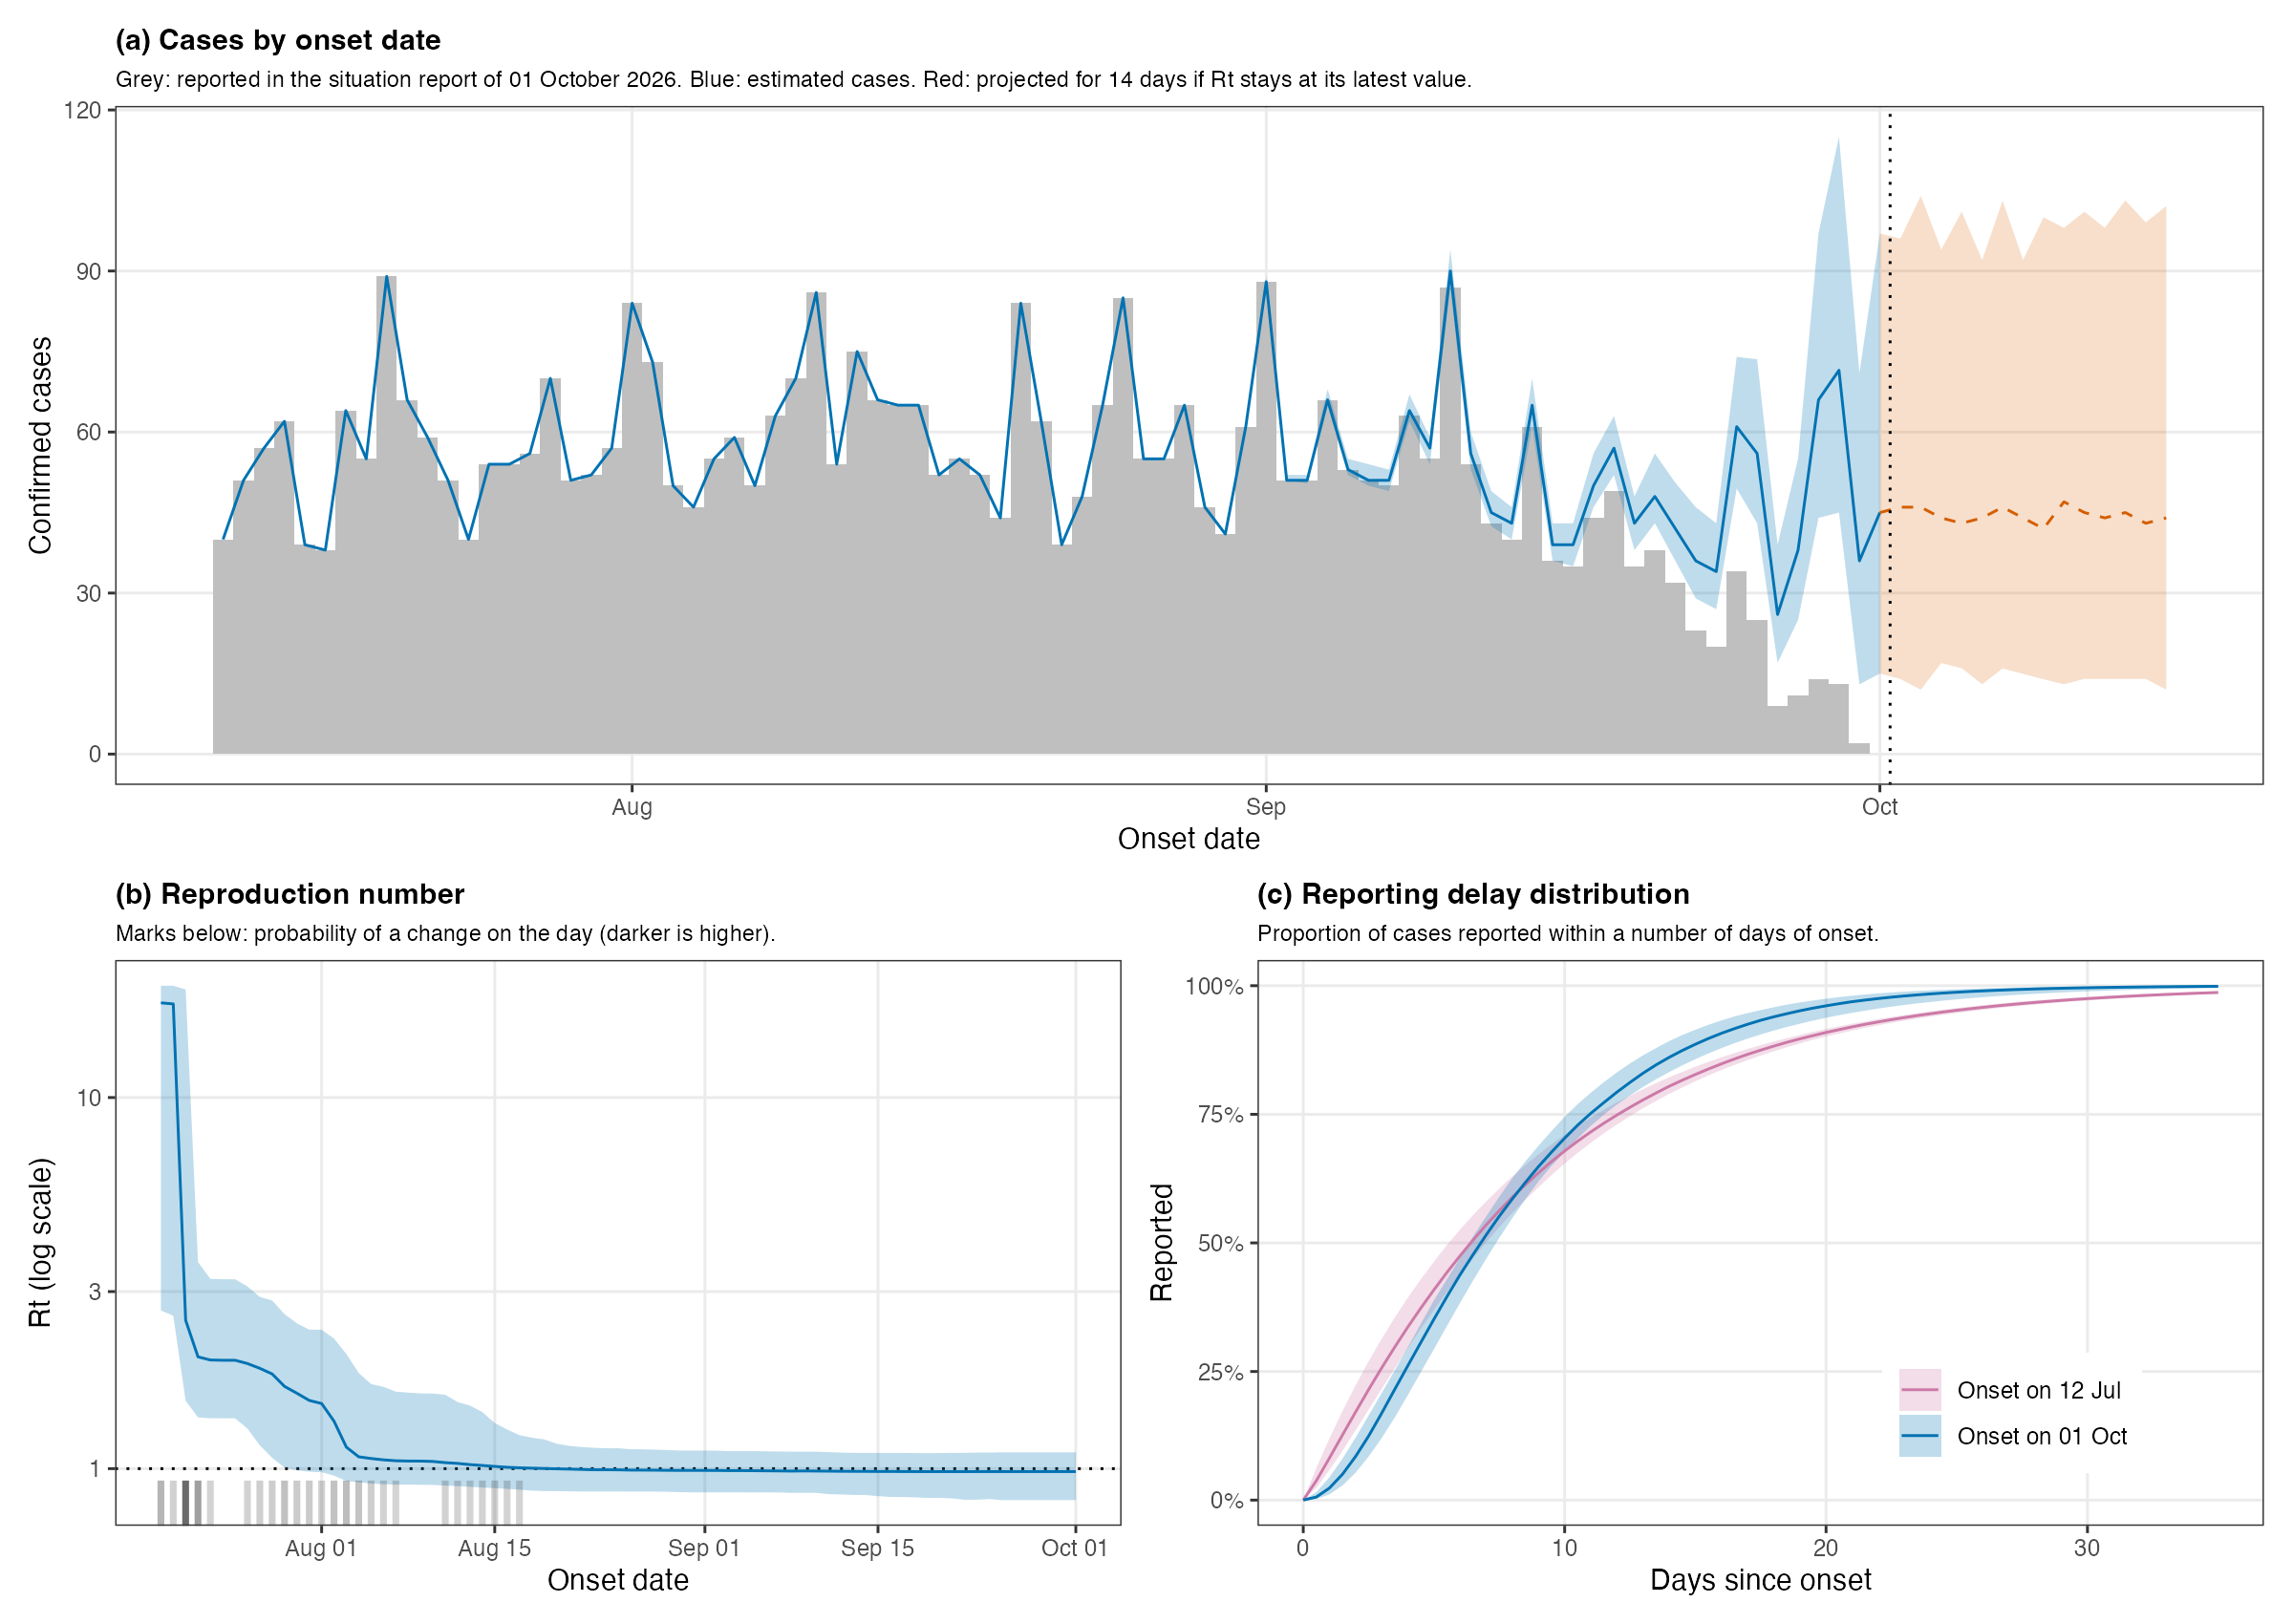
\includegraphics[width=\textwidth]{bvd_changepoint_main.png}
\end{column}
\begin{column}{0.34\textwidth}
\small
\textbf{Cases.} Reported counts fall steeply; estimated cases do not. Last
five onset days: \bvdRecentMedians{} a day (90\% intervals spanning
\bvdRecentInterval).

\medskip
\textbf{$R_t$.} \bvdRtFirst{} in mid-July; \bvdRt{} now. Probability that it
has not changed: \bvdRtNoChange.

\medskip
\textbf{Delay.} Mean \bvdDelayMean{} days.

\medskip
\textbf{Day of week.} Monday \bvdPsiMon; Tuesday \bvdPsiTue.

\medskip
\textbf{Errors.} About \bvdErroneousPerHundred{} per 100 cases reported,
lasting about \bvdErroneousDays{} days.

\medskip
\textbf{Caveats.} Borrowed serial interval; a change in the last week or two
cannot be told from a change in incidence.
\end{column}
\end{columns}
\end{frame}

\end{document}
